\documentclass[11pt]{article}
\usepackage[a4paper,margin=1in]{geometry}
\usepackage[T1]{fontenc}
\usepackage{lmodern,microtype}
\usepackage{amsmath,amssymb,amsthm}
\usepackage{booktabs,array}
\usepackage{xcolor,listings,needspace}
\usepackage{tikz}
\usetikzlibrary{positioning,arrows.meta}
\usepackage[hyphens]{url}
\usepackage[hidelinks]{hyperref}
\definecolor{codegray}{gray}{0.96}
\lstset{language=C++,basicstyle=\ttfamily\small,backgroundcolor=\color{codegray},
 frame=single,framerule=0.2pt,columns=fullflexible,keepspaces=true,
 breaklines=true,showstringspaces=false,tabsize=4}
\newcommand{\clangsolv}{\textsc{ClangSOLV}}
\newcommand{\csolv}{\textsc{CSOLV}}
\newcommand{\jsolv}{\textsc{JSOLV}}
\newcommand{\labels}{\mathcal L}
\newtheorem{proposition}{Proposition}
\title{ClangSOLV: Clang Static Object Labelling for Verification\\
A Standalone Annotation Frontend for Ordinary C++ Values}
\author{Jayanta Majumder \and Sambuddha Majumder}
\date{10 October 2026}
\begin{document}
\maketitle
\begin{abstract}
Workflow facts such as Persisted, Validated and Authenticated describe whether
a value is ready for a particular use, independently of its nominal domain
type. ClangSOLV makes these application-owned facts available as contracts on
ordinary C++ functions and values. A build-time generator registers labels from
a small configuration file. Contract macros attach Clang annotations to
declarations; a standalone LibTooling executable reads the semantic AST, checks
requirements, propagates evidence through assignments and native branches,
and computes fixed points for structured loops. An optional JSON report
records known and missing evidence at consumers. The normal compiler then
produces the executable, with checking enforced as a build prerequisite.
This design restores much of the annotation-oriented experience of JSOLV
without requiring C++ state wrappers or a compiler fork. The implementation
deliberately covers a bounded structured subset of C++ and rejects unmodelled
operations. Its return, preservation and read-only contracts are trusted;
coarse invalidation is conservative but can discard unrelated facts. This
paper presents the architecture, evidence calculus, complete application
pattern, build and reporting interfaces, validation results, and the limits
arising from mutation, copying, aliasing and external context.
\end{abstract}

\section{The motivation: facts alongside ordinary types}
An article may be persisted, validated and authenticated while remaining an
\texttt{Article}. Publication requires all three facts, but its nominal type
alone does not say whether the corresponding workflow stages occurred.
Application programmers usually encode the missing information in comments,
call ordering, runtime flags or numerous wrapper types. A static labelling
layer makes the required evidence visible and checks that every incoming path
supplies it.

The static-property-tag proposal distinguishes value facts from nominal
shape~\cite{tags}. The semantic-category proposal similarly argues for making
architectural intent explicit~\cite{roles}. \jsolv{} implements application-owned
labels as generated Java annotations and propagates their evidence through
a compiler processor~\cite{jsolv}. \csolv{} provides a portable C++17 alternative
using generated label types, state wrappers and native template checks~\cite{csolv}.
That portability is valuable, but explicit wrappers, borrowing views and state
selection place additional structure in application code.

The question motivating \clangsolv{} is whether C++ can offer the more direct
experience: ordinary objects, annotated contracts and automatic evidence flow
through native assignments and branches. The answer developed here is a
standalone Clang-based frontend. This paper is self-contained; the related
implementations provide context rather than prerequisites.

\section{A separate frontend, without a separate C++ parser}
\clangsolv{} links Clang's LibTooling, AST and analysis libraries. It uses Clang
to parse declarations, resolve names and overloads, and instantiate templates.
The tool then applies an evidence analysis to the semantic representation.
LibTooling's standalone-tool pattern supplies the frontend action and access
to compilation settings~\cite{tooling}. The executable performs checking,
not object-code generation, and can be invoked as a mandatory stage before
ordinary compilation.

The distinction between syntax and interpretation matters. C++ attribute
syntax can carry extra tokens, but syntax alone does not implement custom
label checking. \clangsolv{} uses \texttt{clang::annotate}, which Clang documents
as metadata for external static-analysis tools~\cite{annotate}. This is a
Clang-specific facility, even though it uses familiar attribute syntax. The
implementation does not require a compiler fork or a dynamically loaded
plugin, and does not rely on scanning source text or parsing a dumped AST.

The current analysis follows structured AST control flow and validates that
Clang can construct each checked function's control-flow graph (CFG). It is
\emph{not} a general solver over every Clang CFG element and does not use the
Clang flow-sensitive framework as its transfer engine. This choice permits a
small, explicit semantic core, provided that unsupported control-flow and
expression forms produce errors. A future general CFG solver could expand
coverage without changing the contract interface.

\section{Configuration, metadata and build architecture}
The application owns its vocabulary in a small properties file:
\begin{lstlisting}[language={}]
namespace=example::tags
labels=Persisted, Validated, Authenticated, Approved
\end{lstlisting}
The generator emits a header with empty declarations such as:
\begin{lstlisting}
#include <clangsolv/annotations.hpp>
namespace example::tags {
struct CLANGSOLV_ANNOTATE("clangsolv.label") Persisted {};
struct CLANGSOLV_ANNOTATE("clangsolv.label") Validated {};
struct CLANGSOLV_ANNOTATE("clangsolv.label") Authenticated {};
struct CLANGSOLV_ANNOTATE("clangsolv.label") Approved {};
}
\end{lstlisting}
The marker registers the qualified record name as a label identity. Contract
names are resolved against these records: unambiguous short names are
convenient, while qualified names disambiguate vocabularies. A label named
Validated in one namespace does not equal a similarly named label elsewhere.
Adding Approved requires no special checker or library code.

The generator validates identifiers, rejects keywords, duplicate labels and
unknown or repeated keys, and emits one build-tree header. Blank lines and
full-line comments are supported; Java-properties escape and continuation
rules are not. Unchanged output retains its modification time. A successful
regeneration removes declarations deleted from the configuration; malformed
configuration fails the dependent build.

\begin{figure}[ht]
\centering
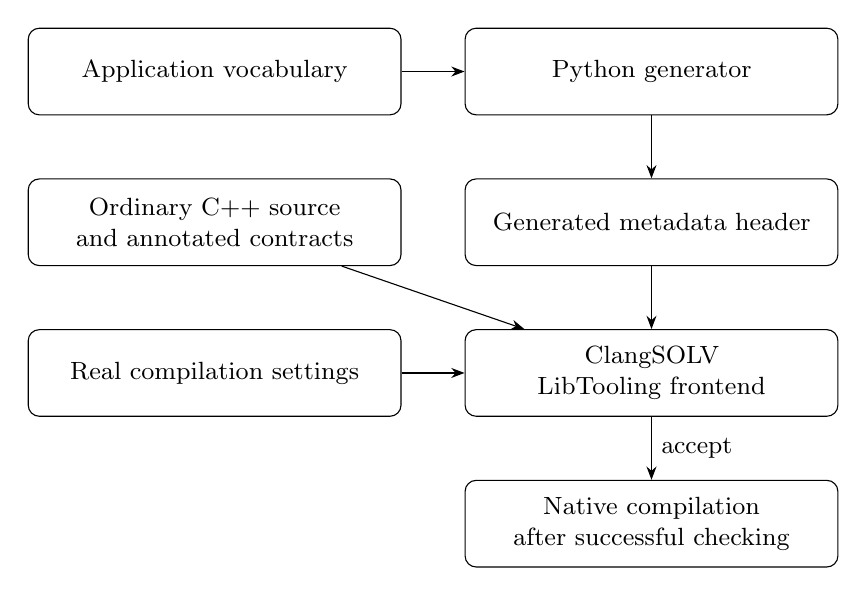
\begin{tikzpicture}[node distance=8mm,
 box/.style={draw,rounded corners,align=center,font=\small,text width=45mm,minimum height=11mm},
 >={Stealth}]
\node[box] (config) {Application vocabulary};
\node[box,right=of config] (generate) {Python generator};
\node[box,below=of generate] (header) {Generated metadata header};
\node[box,left=of header] (source) {Ordinary C++ source\\and annotated contracts};
\node[box,below=of header] (check) {ClangSOLV\\LibTooling frontend};
\node[box,left=of check] (flags) {Real compilation settings};
\node[box,below=of check] (native) {Native compilation\\after successful checking};
\draw[->] (config)--(generate);
\draw[->] (generate)--(header);
\draw[->] (header)--(check);
\draw[->] (source)--(check);
\draw[->] (flags)--(check);
\draw[->] (check)--node[right,font=\small]{accept}(native);
\end{tikzpicture}
\caption{The checking frontend consumes application metadata and real C++
semantics; native compilation is gated by its result.}
\label{fig:architecture}
\end{figure}

\section{The contract interface}
Four macros express the public contract vocabulary:
\begin{table}[ht]
\centering\small
\begin{tabular}{p{0.39\linewidth}p{0.54\linewidth}}
\toprule
Contract & Interpretation\\
\midrule
\texttt{returns(L...)} & Successful return establishes the listed labels.\\
\texttt{needs(L...)} & A parameter needs all the listed labels.\\
\texttt{preserves(k)} & Result retains evidence of argument $k$, indexed from one.\\
\texttt{readonly} & Call promises not to invalidate the caller's tracked evidence.\\
\bottomrule
\end{tabular}
\caption{Contracts attach to ordinary declarations. Returns, preservation and
read-only effects are trusted summaries.}
\end{table}

For example, the return macro expands to an annotation string with a stable
protocol prefix:
\begin{lstlisting}
#define returns(...) \
    [[clang::annotate("clangsolv.returns:" #__VA_ARGS__)]]
\end{lstlisting}
The checker resolves its label names against the registered vocabulary. It
also rejects misplaced contracts, unknown or ambiguous labels, invalid
preservation indices and preservation across unrelated nominal domain types.

An annotated public header is sufficient to communicate contracts across
translation units. The checker gathers function redeclarations and their
parameter metadata, so a definition and a call need not repeat the header's
contracts. This is summary-based checking: it does not infer cross-translation-unit
body effects or prove an implementation's advertised postconditions.

readonly is intentionally separate from preserves. The latter describes the
\emph{returned value}, which can be a distinct object. It does not promise that
the original argument remains usable with its old evidence. A call without
readonly erases the caller's environment after checking arguments and capturing
the result's evidence. A truthful readonly summary allows prior facts to remain.
The promise concerns facts, not absence of output: printing an immutable
snapshot can be read-only in this sense.

\section{Evidence semantics and structured flow}
Let $\labels$ be the set of registered label identities. A checking environment
$E$ maps named automatic variables and reference parameters to subsets of
$\labels$. Missing entries mean no known facts. Requirements use the subset rule
\[
  \operatorname{Require}(R,x,E)\text{ succeeds}\quad\Longleftrightarrow\quad
  R\subseteq E(x).
\]
Declared parameter requirements seed the entry environment inside their
function. Labels remain atomic: the implementation does not infer implications,
negation, parameterised predicates or a policy hierarchy.

\subsection{Calls, initialization and mutation}
If a called function establishes return set $A$ and preserves argument $k$, its
result evidence is $A\cup S_k$, where $S_k$ is that argument's incoming evidence.
The shorthand \texttt{preserves()} defaults to \texttt{preserves(1)};
\texttt{preserves(2)} selects the second explicit argument. The macro emits
an empty index payload for the shorthand, which the checker interprets as one.
Without preservation the result has only $A$. Requirements are checked before
the call's conservative effect erasure. Reference arguments are checked against
their current storage evidence, rather than a stale earlier snapshot.

Initialization binds the expression's evidence to its destination. Direct
assignment first clears the existing environment, then binds the new evidence
to the destination. Member writes, compound assignments, increments and taking
addresses clear the whole environment. Uncontracted calls similarly clear it.
This is a coarse approximation intended to avoid retaining evidence through
unknown alias effects; it can lose facts about unrelated values.

Defaulted copy and move operations can transfer evidence to destinations
under a semantic-fidelity assumption. Moves discard source evidence, and
nontrivial defaulted copies conservatively clear other facts before binding
their result. Custom constructors do not transfer labels implicitly, and
nontrivial constructor effects may clear existing evidence. Consequently,
raw branch destinations should be constructed before evidence-bearing stages
in the current frontend. Member/element reads do not inherit their container's
labels, and type-changing conversions do not transfer evidence.

Direct reference aliases share a named variable's evidence region. More
complex reference bindings have conservative independent bindings; later
writes or unknown calls still clear all facts. Global and static-local storage
is not tracked, and labelled pointer contracts are rejected. This model is
not a general pointer or memory-region analysis.

\subsection{Branches, short circuits and early exits}
For reachable normal paths, the join is pointwise intersection:
\[
 (E_1\sqcap E_2)(x)=E_1(x)\cap E_2(x).
\]
An \texttt{if} analyses both alternatives and joins their normal, break and
continue exits separately. A return or standalone throw ends its current normal
path, so it contributes no facts to later normal execution. A conditional
expression computes both the environment join and the intersection of its
possible result labels. A short-circuit operator joins the executed and
skipped right-hand paths. No predicate solver or literal-condition pruning
is implemented; even constant conditions receive conservative treatment.

\subsection{Loops and the danger of the first-iteration assumption}
A loop must not check its body using only the facts available on its first
iteration. For example, a body can consume a persisted article and then edit
it; later iterations no longer have the original persistence evidence.

For entry environment $E$ and loop head $H$, the engine repeatedly computes
\[
 H_{n+1}=E\sqcap\operatorname{Back}(H_n),\qquad H_0=E,
\]
where Back joins normal and continue paths and applies increment and condition
effects where appropriate. Requirements are diagnosed at the stable head,
not during exploratory iteration. Break states contribute directly to the
loop's exits. \texttt{while} and \texttt{for} include zero iterations; a
\texttt{do} loop executes its body at least once.

The finite evidence domain supports descending fixed-point iteration for
the supported transfer model. A safety limit of 1024 iterations rejects
unexpected nonconvergence. Nested loops use the same mechanism. Loop condition
declarations are explicitly unsupported in the initial implementation.

\section{Explicit proof points and revocation}
The annotation header also supplies runtime no-op templates operating on
ordinary named values:
\begin{lstlisting}
clangsolv::establish<Persisted, Validated>(article);
clangsolv::require<Persisted>(article);
clangsolv::forget<Validated>(article);
clangsolv::forget(article); // discard every known label
\end{lstlisting}
Establishment unions trusted application evidence, requirement checks a subset,
and forgetting removes selected facts or all facts. Only registered label
types are accepted. These markers do not validate business predicates or
allocate runtime label storage. They must name automatic values or reference
parameters; unnamed expressions, pointers, global and static-local storage are
not supported targets.

The explicit establishment marker is a trust boundary, not a loophole to be
used wherever a diagnostic is inconvenient. It belongs after an audited
domain action has supplied the fact. Selective forgetting supports revocation
without altering the underlying value, useful when a programmer elects to
stop relying on a fact even though the object itself is unchanged.

\Needspace{18\baselineskip}
\section{A self-contained publishing example}
After generating the example vocabulary above, concatenating the following
three listings produces a complete program. The first declares ordinary
domain data and public contracts:
\begin{lstlisting}
#include <clangsolv_labels.hpp>
#include <iostream>
#include <stdexcept>
#include <string>
#include <vector>
using namespace example::tags;
struct Article { std::string title; };

returns(Persisted)
Article persist(Article article);
readonly returns(Validated)
preserves()
Article validate(const Article& article);
readonly returns(Authenticated)
preserves()
Article authenticate(const Article& article,
                     const std::string& credential);
readonly
void publish(needs(Persisted, Validated, Authenticated)
             const Article& article);
\end{lstlisting}
The implementations supply the domain work. Their return and effect contracts
are trusted; ClangSOLV does not prove the database or authentication semantics.
Here storage is an in-process demonstration rather than durable persistence.

\Needspace{24\baselineskip}
\begin{lstlisting}
Article persist(Article article) {
    static std::vector<Article> store;
    store.push_back(article);
    return article;
}
Article validate(const Article& article) {
    if (article.title.empty()) throw std::invalid_argument("empty title");
    return article;
}
Article authenticate(const Article& article,
                     const std::string& credential) {
    if (credential != "demo-author")
        throw std::invalid_argument("invalid credential");
    return article;
}
void publish(const Article& article) {
    std::cout << article.title << '\n';
}
\end{lstlisting}
The client code uses native declarations, branches and assignments:
\Needspace{26\baselineskip}
\begin{lstlisting}
int main(int argc, char**) {
    Article chosen; // raw construction before gathering evidence
    const std::string credential="demo-author";
    const auto saved=persist(Article{"Plain objects, checked facts"});
    const auto checked=validate(saved);
    const auto ready=authenticate(checked,credential);
    publish(ready);

    if (argc>1) chosen=checked;
    else chosen=saved;
    clangsolv::require<Persisted>(chosen); // common evidence
    const auto checkedAgain=validate(chosen);
    const auto readyAgain=authenticate(checkedAgain,credential);
    publish(readyAgain);

    clangsolv::establish<Approved>(chosen); // audited demo assertion
    clangsolv::require<Approved>(chosen);
    clangsolv::forget<Approved>(chosen);
}
\end{lstlisting}
The two branch alternatives have Persisted in common. Only one has Validated,
so the join loses validation evidence; subsequent stages regain it. Approved
demonstrates vocabulary extension and explicit proof markers. Authentication's
credential is bound beforehand to avoid a side-effecting temporary construction
in a multi-argument preservation call.

The repository application separates these declarations and implementations
into a public workflow header, implementation source and main source. Its
mandatory checking step covers both translation units before native compilation.

\section{Failures that a normal compiler would accept}
Ordinary C++ compilation accepts the following function calls because every
argument has the expected nominal type. ClangSOLV supplies the missing workflow
discipline:
\begin{lstlisting}
auto saved=persist(draft);
publish(saved); // missing Validated and Authenticated
\end{lstlisting}
After gathering all three facts, mutation invalidates them:
\begin{lstlisting}
ready.title="Changed after checking";
publish(ready); // old evidence has been discarded
\end{lstlisting}
A branch cannot lend facts known only on one path:
\begin{lstlisting}
if (condition) chosen=checked;
else chosen=saved;
clangsolv::require<Validated>(chosen); // not common to both paths
\end{lstlisting}
Nor can a loop retain first-iteration evidence after a write:
\begin{lstlisting}
while (condition) {
    clangsolv::require<Persisted>(article);
    article.title="Edited inside the loop";
} // requirement also has to hold on later iterations
\end{lstlisting}
The application contains four separate, deliberately rejected translation
units covering these cases. They are excluded from the successful native
build and exercised by a rejection test. Diagnostics name the consumer,
missing labels, known labels and source location.

\section{Build gating, compilation databases and reports}
The reusable tool is in \path{.}, and the showcase
is in \path{example-app}. Building the checker requires
matching LLVM and Clang development libraries and headers, a compatible host
compiler, CMake 3.20 or newer and Python 3.10 or newer. A compiler-only Clang
installation is insufficient for building a LibTooling executable.

Typical commands are:
\begin{lstlisting}[language={}]
cmake -S . -B tool-build \
  -DLLVM_DIR=/path/to/lib/cmake/llvm \
  -DClang_DIR=/path/to/lib/cmake/clang
cmake --build tool-build --config Release
ctest --test-dir tool-build -C Release --output-on-failure
\end{lstlisting}
These line continuations are for POSIX shells; PowerShell users can place each
command on one line. The companion usage guide records the tested Windows
Visual Studio configure command and its LLVM installation paths.

The CMake helper makes generation and checking prerequisites of native
compilation:
\begin{lstlisting}[language={}]
include(path/to/clangsolv/cmake/ClangSOLV.cmake)
add_executable(my_app main.cpp workflow.cpp)
clangsolv_enable(my_app clangsolv.properties
  CHECKER "/absolute/path/to/clangsolv"
  SOURCES main.cpp workflow.cpp
  OPTIONS "-I${CMAKE_CURRENT_SOURCE_DIR}/include"
  DEPENDS include/workflow.hpp)
\end{lstlisting}
The helper always rechecks when the target builds, avoiding a stale success
stamp after header changes. Compilation flags in OPTIONS must match the
application; the initial helper does not infer arbitrary CMake target settings.
For complex builds, LibTooling's compilation-database interface is preferable:
\begin{lstlisting}[language={}]
clangsolv -p myapp/build --report myapp/build/check.json \
  myapp/main.cpp myapp/workflow.cpp
\end{lstlisting}
The database supplies working directories and actual compile arguments rather
than guessed include paths~\cite{database}. Every relevant translation unit
must be checked. Standalone explicit flags are also accepted after
\texttt{--}. Clang must be able to parse those flags and the backend's headers.

The report records overall acceptance, native frontend exit status, checked
function and CFG counts, files, checker diagnostics and requirement events.
A requirement event includes:
\begin{lstlisting}[language={}]
"consumer": "example::publish",
"required": ["example::tags::Authenticated",
             "example::tags::Persisted", "example::tags::Validated"],
"known": ["example::tags::Persisted"],
"missing": ["example::tags::Authenticated", "example::tags::Validated"],
"accepted": false
\end{lstlisting}
Location fields accompany this data. Clang's parser diagnostics remain on
stderr; parser failure rejects the overall report but is not duplicated in
the checker-specific diagnostic array. Reports describe evidence at checked
consumers, not an independently verified domain proof.

On a non-Clang native backend, macros erase to ordinary declarations. This
permits GCC or MSVC to generate executable code, but compilation by those
backends alone does not enforce these contracts. Mandatory checking is
therefore part of the design, whereas the portable CSOLV template library's
requirements remain native type checks.


\section{Labels on smart-pointer pointees}
The same interface now supports ordinary \texttt{std::shared\_ptr<T>} and
\texttt{std::unique\_ptr<T>} with the default deleter. Labels describe the
managed object of type T, not the ownership wrapper. Semantic recognition of
standard-library template specialisations also recognises application type
aliases. No wrapper type is inserted into the template argument list.

\begin{lstlisting}
returns(Persisted)
std::shared_ptr<Article> persistShared(Article draft);
readonly returns(Validated) preserves()
std::shared_ptr<Article> validateShared(
    const std::shared_ptr<Article>& article);
readonly void inspect(
    needs(Persisted, Validated) const Article& article);

void pointerWorkflow() {
    auto saved = persistShared(Article{"Draft"});
    auto checked = validateShared(saved);
    auto alias = checked;
    inspect(*alias);
    clangsolv::require<example::tags::Validated>(alias);
}
\end{lstlisting}

A requirement on a smart-pointer parameter checks its pointee evidence; a
return contract establishes evidence on the returned pointee. Preservation
compares underlying domain types, ignoring ownership wrappers and const
qualification. Dereference and arrow access transfer the known evidence.
Proof markers on a named smart pointer likewise describe its managed object;
establishment is a trusted assertion of a live pointee satisfying the labels.
Default or empty pointers carry no evidence. Labels do not independently prove
nullness or lifetime safety.

The analysis deliberately retains the finite environment model rather than
introducing a heap graph. A shared-pointer copy inherits its source's currently
known evidence snapshot. A unique-pointer move transfers evidence to the new
owner and invalidates the source; the conservative implementation also erases
other tracked facts. Mutation, reset, swap, assignment, get, release and unknown
calls erase the whole environment, including facts on copied handles and
borrowed references. Assignment currently restores no smart-pointer evidence;
initialisation from a contracted factory is preferred. Forgetting erases other
variables' evidence before retaining unforgotten labels on its named target.
Const ownership observers preserve facts. Branch and loop intersections apply
unchanged.

This simple policy is safe against modelled alias mutations but intentionally
imprecise: establishing a label after copying a handle does not automatically
label the earlier copy. Preservation promises result facts, not object identity.
It therefore needs no inference that a contracted function returns the same
allocation. The runnable application contains a separate smart-pointer showcase.

Arrays, nested pointer pointees, custom unique-pointer deleters, raw-pointer
adoption and converting ownership constructors are rejected. Creation uses
make\_shared, make\_unique or a trusted contracted factory. Such factory summaries
must exclude hidden disposal effects on other tracked objects, including custom
shared-pointer deleters. Visible user-defined pointee destructors are rejected.
Concurrent mutation, invisible external alias effects and general lifetime
analysis remain outside this sequential trusted-contract model. Raw-pointer
contracts remain unsupported.

\section{Scope, trust and precision}
Supported structured control flow includes blocks, declarations, expressions,
if/else, conditional expressions, while/for/do, break/continue, return and
standalone throw. Direct calls and matching-domain preservation are supported.
Available nondependent user function bodies, including header bodies, are
analysed. Instantiated templates are visited; uninstantiated dependent bodies
are deferred. System-header implementations are treated as opaque boundaries.

The initial frontend rejects switch, goto, range-for, try/catch, coroutines,
lambdas, indirect calls, virtual dispatch, dangerous casts and unmodelled AST
expressions. Direct construction of user-custom-destructor objects is rejected;
this does not establish a complete cleanup analysis for objects managed inside
libraries. Side-effecting multi-argument calls with requirements or preservation
are rejected rather than analysed in an assumed argument order. These are
explicit scope restrictions, not missing syntax in the native language.

Multiple side-effecting arguments and unsequenced side-effecting binary operands
are also rejected, including nested contract calls. Binding results first makes
their order explicit. Contracts on member operators count explicit parameters;
the frontend accounts separately for Clang's implicit receiver argument.

Return establishment, preservation and readonly are trusted application
summaries. The implementation does not inspect their bodies to prove the
advertised postconditions. Defaulted copying and moving are also assumed to
transfer the meaning of relevant value facts; custom member operations can
violate that assumption. Mutable members, pointers inside records, aliases
outside the analysed function, hidden library callbacks, concurrency and
external services can invalidate a semantic fact. No general whole-program
soundness, lifetime, memory-safety or authentication theorem is claimed.

Within the supported transfer model, intersection ensures that a branch join
does not introduce a fact unavailable on another incoming normal path. Loop
fixed points prevent first-iteration knowledge being reused indefinitely.
These useful properties must be distinguished from proving that an introduced
fact is true in the application domain.

Coarse erasure is intentionally conservative. An increment of an unrelated
counter or an unmodelled nontrivial constructor can discard an article's
evidence. The application demonstrates constructing raw branch storage before
gathering evidence and using small, truthful contracted boundaries. readonly
must not be attached merely to silence a diagnostic. Region-sensitive effects,
a general CFG solver and verified summaries would improve precision and
coverage; none is needed to extend the vocabulary.

\section{Validation and the relationship between the frontends}
The checker is built against LLVM/Clang 19.1.0 using MSVC 19.44 on Windows.
Its 60-test suite exercises actual LibTooling invocations, rather than mocked
ASTs or source-text matching. Cases cover accumulation and missing requirements,
replacement, copies and moves, aliases, early returns, joins, short circuits,
loops, explicit proof markers, label extension, namespace ambiguity, instantiated
templates, malformed contracts, unsupported operations, parser rejection,
compilation databases and generation behaviour. The application adds runtime
execution and four deliberately rejected workflow examples.

The checked application compiles and runs using both native MSVC and GCC
13.3.0. These results establish working separation between analysis and code
generation in this environment, not validation of every LLVM version or
platform. LLVM/Clang 18 and newer is the intended API range; the measured
implementation is 19.1.0. Its development package contained an obsolete absolute
DIA SDK link dependency, handled through local CMake target rebinding without
editing the installed package.

\begin{table}[ht]
\centering\small
\begin{tabular}{>{\raggedright\arraybackslash}p{0.19\linewidth}>{\raggedright\arraybackslash}p{0.22\linewidth}>{\raggedright\arraybackslash}p{0.22\linewidth}>{\raggedright\arraybackslash}p{0.22\linewidth}}
\toprule
Aspect & JSOLV & CSOLV & ClangSOLV\\
\midrule
Application values & Ordinary Java values & Explicit C++ state wrappers & Ordinary C++ values\\
Contract carrier & Generated annotations & Template label sets & Generated metadata and annotations\\
Checking engine & Java processor & Native type checker & Standalone Clang frontend\\
Branch join & Analysed flow & Explicit selection & Analysed structured flow\\
Build obligation & Processor enabled & Normal compilation & Mandatory checking stage\\
\bottomrule
\end{tabular}
\caption{Shared evidence philosophy, different enforcement mechanisms.}
\end{table}
\clangsolv{} moves the C++ application experience closer to \jsolv{}, while
\csolv{} remains attractive for compiler-independent type enforcement. All
three use application-owned facts and trusted introduction boundaries. Their
interfaces need not be forced into one representation to share that philosophy.

\section{Conclusion}
\clangsolv{} shows that ordinary C++ values can carry a practical static
workflow discipline through a standalone annotation frontend. The vocabulary
is configuration-owned, contracts are visible in public declarations, and
native assignments, branches and supported loops propagate evidence. Real
Clang semantics provide the parsing foundation; mandatory build gating makes
the additional verification effective. The bounded analysis and explicit
trust model keep the implementation's claims proportionate to its behaviour,
while leaving a clear path toward broader control-flow and effect support.

\begin{thebibliography}{9}
\raggedright
\bibitem{tags} S. Majumder and J. Majumder.
\emph{User-Defined Static Property Tags for Mainstream Programming Languages:
A Lightweight Flow-Sensitive Verification Layer}. Companion manuscript,
\texttt{static\_property\_tags.tex}.
\bibitem{roles} J. Majumder and S. Majumder.
\emph{Explicit Semantic Categories for More Legible Mainstream Programming Languages}.
Companion manuscript, \texttt{semantic\_roles\_beyond\_class.tex}.
\bibitem{jsolv} J. Majumder and S. Majumder.
\emph{JSOLV: Java Static Object Labelling for Verification}.
Companion manuscript, \texttt{jsolv.tex}, 2026.
\bibitem{csolv} J. Majumder and S. Majumder.
\emph{CSOLV: C++ Static Object Labelling for Verification}.
Companion manuscript, \texttt{csolv.tex}, 2026.
\bibitem{tooling} LLVM Project.
Tutorial for building tools using LibTooling and LibASTMatchers.
\url{https://clang.llvm.org/docs/LibASTMatchersTutorial.html}.
\bibitem{annotate} LLVM Project. Clang attribute reference: annotate.
\url{https://clang.llvm.org/docs/AttributeReference.html#annotate}.
\bibitem{database} LLVM Project. JSON compilation database format specification.
\url{https://clang.llvm.org/docs/JSONCompilationDatabase.html}.
\end{thebibliography}
\end{document}
